\chapter{Arhitektura i dizajn sustava}
		
		
	\noindent Arhitektura prati model klijent – server koja omogućava fleksibilnost u razvoju i održavanju budući da backend i frontend mogu evolouirati neovisno jedno o drugome. Komunikacija se vrši putem HTTP protokola.
	React je korišten za izgradnju frontend-a (klijentske strane), Spring Boot kao backend server, a PostgreSQL kao sustav za upravljanje bazom podataka. Pri izradi korisničkog sučelja komponente su građene tako da su reaktivne i ažuriraju se automatski kada se stanje aplikacije promijeni. Za upravljanje navigacijom unutar aplikacije korišten je React Router.
	Spring Boot je korišten za izradu backend dijela aplikacije koji obuhvaća:
	
	\begin{itemize}
		\item poslovnu logiku - servisi komuniciraju s repozitorijima i drugim servisima kako bi izvršili operacije nad podacima
		\item RESTful API-je - Rest Controlleri su definirani kako bi se obradili API zahtjevi, mapirani kao RESTful endpointovi
		\item pristup PostgreSQL bazi podataka – za komunikaciju se definiraju JPA repozitoriji koji omogućavaju pristup i upravljanje podacima.
	\end{itemize}
	
	
	Korisnik putem WEB preglednika šalje zahtjev WEB poslužitelju. WEB poslužitelj omogućava komunikaciju između klijenta i aplikacije putem HTTP protokola. Ukratko, WEB poslužitelj pokreće aplikaciju te joj prosljeđuje korisnikove zahtjeve. Frontend šalje HTTP zahtjeve prema SpringBootu putem fetcha, a backend obrađuje zahtjeve, pristupa bazi podataka, izvršava logiku i vraća rezultat frontendu u obliku JSON objekta.  Aplikacija u konačnici vraća odgovor u obliku HTML dokumenta.
	
		\begin{figure}[H]
		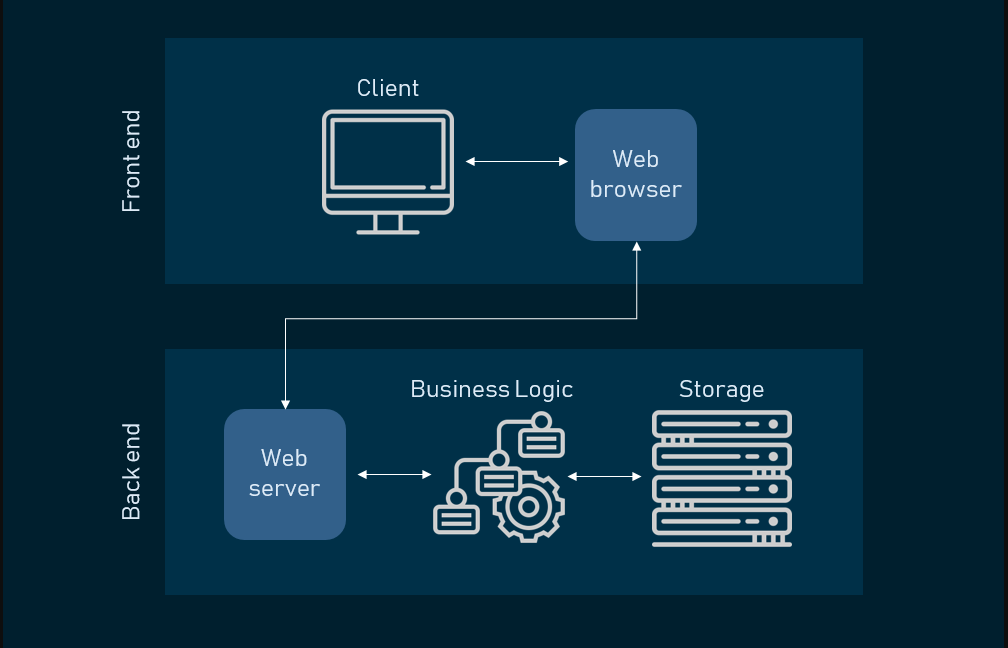
\includegraphics[scale=0.5]{slike/komunikacija.png} %veličina u odnosu na širinu linije
		\centering
		\caption{Komunikacija između frontenda i backenda}
		\label{fig:komunikacija} %label mora biti drugaciji za svaku sliku
		\end{figure}
	
				
		\section{Baza podataka}
			
				\noindent Za potrebe našeg sustava koristit ćemo relacijsku bazu podataka koja svojom strukturom olakšava modeliranje stvarnog svijeta. Temeljna jedinica baze je relacija, odnosno tablica koja je definirana svojim imenom i skupom atributa. Glavna svrha baze podataka je brza i jednostavna pohrana, izmjena i dohvaćanje podataka za daljnju obradu. Baza podataka ove aplikacije sastoji se od sljedećih entiteta:
				
				\begin{itemize}
					\item USER
					\item RESEARCHER
					\item MANAGER
					\item TRACKER
					\item ANIMAL
					\item STATION
					\item ACTION
					\item ACTION\_ANIMAL
					\item TASK
					\item MEDIUM
					\item QUALIFICATION
					\item TRACKER\_HISTORY
					\item ANIMAL\_HISTORY
					\item ROUTE
					\item ROUTE\_POINT
					\item ANIMAL\_COMMENT
					\item ACTION\_COMMENT
					\item ACTION\_HABITAT
					\item CONFIRMATION\_TOKEN
					\item HABITAT
					\item REQUEST
					\item REQUIREMENTS
					\item SPECIES
					\item TASK\_ANIMAL
					\item TASK\_COMMENT
					\item TRACKER\_ACTION\_MEDIUM
				\end{itemize}
				
		\subsection{Opis tablica}
				
				
				\noindent \textbf{USER} \hspace{1em} Ovaj entitet sadržava sve važne informacije vezane za korisnika aplikacije. Sadrži atribute ID korisnika, korisničko ime korisnika u aplikaciji, fotografiju korisnika, šifru računa korisnika, pravo ime i prezime korisnika, e-mail adresu, tip korisnika (istraživač, tragač ili voditelj stanice) i atribut koji označava je li korisnik registriran tipa BOOLEAN.  Ova klasa sadrži zajedničke atribute sva tri tipa korisnika aplikacije (voditelj, istraživač, tragač) te služi za lakše spremanje podataka koje svaki korisnik mora imati. Ovaj entitet je u vezi \textit{One-to-One} sa svakim tipom korisnika aplikacije. S klasom MAP\_COMMENT je u vezi \textit{One-to-Many} jer više korisnika (mora biti istraživač ili tragač) može ostaviti komentar na mapi.
				
				
				\begin{longtblr}[
					label=none,
					entry=none
					]{
						width = \textwidth,
						colspec={|X[6,l]|X[6, l]|X[20, l]|}, 
						rowhead = 1,
					} %definicija širine tablice, širine stupaca, poravnanje i broja redaka naslova tablice
					\hline \SetCell[c=3]{c}{\textbf{USER}}	 \\ \hline[3pt]
					\SetCell{LightGreen}id & INT	&  	jedinstveni identifikator (TRACKER.id ili MANAGER.id ili RESEARCHER.id)  	\\ \hline
					username & VARCHAR &   korisničko ime 	\\ \hline 
					photo & BYTEA & fotografija korisnika 	\\ \hline
					password & VARCHAR	& šifra korisničkog računa \\ \hline
					name & VARCHAR	& ime korisnika \\ \hline
					surname & VARCHAR & prezime korisnika \\ \hline
					email & VARCHAR & e-mail korisnika  \\ \hline 
					role & VARCHAR & tip korisnika  \\ \hline
					registered & BOOLEAN & oznaka koja definira je li korisnik registriran  \\ \hline
				\end{longtblr}
				
				
				\noindent \textbf{RESEARCHER} \hspace{1em} Ovaj entitet sadrži dodatni atribut odobrenja koji je potreban korisniku koji se odlučio za ulogu istraživača u aplikaciji. Povezan je s klasom USER vezom \textit{One-to-One} preko ID ključa. Dodatni atribut nam govori je li korisnik odobren kao istraživač od strane administratora jer je to preduvjet za obavljanje te uloge. U vezi je \textit{One-to-Many} s klasom ACTION (svaki istraživač može organizirati više radnih akcija). Također je s klasom ANIMAL\_COMMENT indirektno preko USER.id u vezi \textit{One-to-Many} jer više istraživača može ostaviti komentar na nekoj životinji.
				
				\begin{longtblr}[
					label=none,
					entry=none
					]{
						width = \textwidth,
						colspec={|X[6,l]|X[6, l]|X[20, l]|}, 
						rowhead = 1,
					} %definicija širine tablice, širine stupaca, poravnanje i broja redaka naslova tablice
					\hline \SetCell[c=3]{c}{\textbf{RESEARCHER}}	 \\ \hline[3pt]
					\SetCell{LightGreen}id & INT &	identifikator istraživača (USER.id)	\\ \hline
					approved & BOOLEAN & oznaka je li istraživač odobren od strane administratora\\ \hline
				\end{longtblr}				
				
				
				\noindent \textbf{MANAGER} \hspace{1em} Ovaj entitet sadrži dodatne atribute koji opisuju korisnika koji ima ulogu voditelja neke stanice. Moguće je da voditelj vodi samo jednu stanicu i također da jedna stanica ima samo jednog voditelja i zato je veza klase STATION i MANAGER \textit{One-to-One}. Dodatni atribut approved  označava je li korisniku odobren zahtjev za ulogu voditelja od strane administratora (isto kao kod istraživača) te atribut idStation označava jedinstveni identifikator stanice kojoj je korisnik voditelj.
				
				
				\begin{longtblr}[
					label=none,
					entry=none
					]{
						width = \textwidth,
						colspec={|X[6,l]|X[6, l]|X[20, l]|}, 
						rowhead = 1,
					} %definicija širine tablice, širine stupaca, poravnanje i broja redaka naslova tablice
					\hline \SetCell[c=3]{c}{\textbf{MANAGER}}	 \\ \hline[3pt]
					\SetCell{LightGreen}id & INT & jedinstveni identifikator (USER.id) \\ \hline
					approved & BOOLEAN & oznaka odobrenja \\ \hline
					\SetCell{LightBlue}idStation & INT & identifikator stanice (STATION.id) \\ \hline
				\end{longtblr}
				
				
				\noindent \textbf{TRACKER} \hspace{1em} Ovaj entitet označava korisnika koji obavlja ulogu tragača. Povezan je vezama \textit{One-to-One} s klasom USER i klasom TRACKER\_ACTION\_MEDIUM koja označava tragača koji trenutno obavlja zadatke neke akcije i vozilo kojim se koristi, te vezom \textit{Many-to-One} s klasom STATION i vezom \textit{One-to-Many} s klasom TASK jer jedan tragač može imati više zadataka. Tragač može obavljati zadatke koji su zadani od strane istraživača samo na jednoj stanici, dok stanica može imati više tragača na različitim zadatcima. S klasom ANIMAL\_COMMENT je indirektno preko USER.id u vezi \textit{One-to-Many} jer više tragača može ostaviti komentar na nekoj životinji. Sadrži atribute longitude i latitude koji služe za čuvanje zadnje poznate lokacije tragača.  Također je u vezi \textit{Many-to-Many} s klasom MEDIUM što se razrješava tablicom QUALIFICATION.
				
				\begin{longtblr}[
					label=none,
					entry=none
					]{
						width = \textwidth,
						colspec={|X[6,l]|X[6, l]|X[20, l]|}, 
						rowhead = 1,
					} %definicija širine tablice, širine stupaca, poravnanje i broja redaka naslova tablice
					\hline \SetCell[c=3]{c}{\textbf{TRACKER}}	 \\ \hline[3pt]
					\SetCell{LightGreen}id & INT & jedinstveni identifikator tragača (USER.id) \\ \hline
					longitude & DOUBLE & geografska dužina \\ \hline
					latitude & DOUBLE & geografska širina \\ \hline
					\SetCell{LightBlue} idStation & INT & jedinstveni identifikator stanice (STATION.id)\\ \hline
				\end{longtblr}
				
				\noindent \textbf{ANIMAL} \hspace{1em} Ovaj entitet predstavlja klasu životinja i sadrži sve atribute koji opisuju neku životinju. Sadrži atribute ID životinje, ID  vrste životinje, fotografiju životinje, ime jedinke, podatke o lokaciji i tekst koji opisuje životinju. U vezi je \textit{One-to-Many} s klasom  TASK jer na nekom zadatku se može pratiti jedna životinja dok više zadataka može pratiti istu životinju. S klasom ANIMAL\_COMMENT je u vezi \textit{One-to-Many} jer više komentara se može ostaviti za istu životinju. U \textit{One-to-Many} vezi je s klasom ANIMAL\_HISTORY koja sprema podatke o kretanju životinje. Također je u \textit{One-to-Many} vezi s klasom ACTION\_ANIMAL gdje se može vidjeti u kojim akcijama je životinja praćena. Još je u \textit{Many-to-Many} vezi s klasom ACTION što se dodatno razrješava u tablici ACTION\_ANIMAL.
				
				
				\begin{longtblr}[
					label=none,
					entry=none
					]{
						width = \textwidth,
						colspec={|X[6,l]|X[6, l]|X[20, l]|}, 
						rowhead = 1,
					} %definicija širine tablice, širine stupaca, poravnanje i broja redaka naslova tablice
					\hline \SetCell[c=3]{c}{\textbf{ANIMAL}}	 \\ \hline[3pt]
					\SetCell{LightGreen}id & INT & jedinstveni identifikator \\ \hline
					speciesId & INT & vrsta životinje \\ \hline
					photo & BYTEA & fotografija životinje \\ \hline
					description & TEXT & opis životinje \\ \hline
					longitude & DOUBLE & geografska dužina \\ \hline
					latitude & DOUBLE & geografska širina \\ \hline
					name & VARCHAR & ime jedinke \\ \hline
				\end{longtblr}
				
				
				
				\noindent \textbf{STATION} \hspace{1em} Ovaj entitet predstavlja klasu stanice koja sadrži atribute koje opisuju stanicu; ID stanice, ime stanice, podatke o lokaciji te kratki opis stanice. U vezi je \textit{One-to-One} s klasom MANAGER jer je za svaku stanicu zadužen je točno jedan voditelj te je u vezi \textit{One-to-Many} s klasom TRACKER jer više tragača može raditi za istu stanicu.
				
				\begin{longtblr}[
					label=none,
					entry=none
					]{
						width = \textwidth,
						colspec={|X[6,l]|X[6, l]|X[20, l]|}, 
						rowhead = 1,
					} %definicija širine tablice, širine stupaca, poravnanje i broja redaka naslova tablice
					\hline \SetCell[c=3]{c}{\textbf{STATION}}	 \\ \hline[3pt]
					\SetCell{LightGreen}id & INT & jedinstveni identifikator stanice \\ \hline
					longitude & DOUBLE & geografska dužina \\ \hline
					latitude & DOUBLE & geografska širina \\ \hline
					name & VARCHAR & ime stanice \\ \hline
					description & TEXT & opis stanice \\ \hline
				\end{longtblr}
				
				
				\noindent \textbf{ACTION} \hspace{1em} Ovaj entitet sadržava sve važne informacije vezane za akciju koju provodi određeni istraživač. Sadrži atribute ID, naslov, ID istraživača koji provodi akciju, ID voditelja postaje gdje se odvija akcija, vrijeme početka, vrijeme kraja te status  za trenutno stanje akcije (čeka da postane aktivna, na čekanju, riješena). Ovaj entitet u vezi je \textit{Many-to-One} s entitetom RESEARCHER preko ID-a istraživača te je u vezi \textit{One-to-Many} s entitetima TASK koji predstavlja zadatak, TRACKER\_ACTION\_MEDIUM koji predstavlja trenutno aktivne tragače u akcijama te njihov način prijevoza, ANIMAL\_COMMENT koji predstavlja komentar tragača vezan za određenu životinju u nekoj akciji te ACTION\_ANIMAL gdje se može vidjeti koje životinje se prate u akciji. Još je u \textit{Many-to-Many} vezi s entitetom HABITAT te ANIMAL što se dodatno razrješava u tablici ACTION\_ANIMAL.
				
				\begin{longtblr}[
					label=none,
					entry=none
					]{
						width = \textwidth,
						colspec={|X[6,l]|X[6, l]|X[20, l]|}, 
						rowhead = 1,
					} %definicija širine tablice, širine stupaca, poravnanje i broja redaka naslova tablice
					\hline \SetCell[c=3]{c}{\textbf{ACTION}}	 \\ \hline[3pt]
					\SetCell{LightGreen}id & INT & jedinstveni identifikator \\ \hline
					title & VARCHAR & naslov akcije \\ \hline
					\SetCell{LightBlue}idResearcher & INT & ID istraživača (RESEARCHER.id) \\ \hline
					\SetCell{LightBlue}idManager & INT & ID voditelja postaje (MANAGER.id) \\ \hline
					startOfAction & TIMESTAMP & vrijeme početka \\ \hline
					endOfAction & TIMESTAMP & vrijeme kraja \\ \hline
					status & INT & kodni broj za trenutno stanje akcije \\ \hline
				\end{longtblr}
				
				
				\noindent \textbf{ACTION\_ANIMAL} \hspace{1em} Ovaj entitet sadržava sve važne informacije vezane za praćene životinje u nekoj akciji te razrješava \textit{Many-to-Many} vezu između entiteta ANIMAL i ACTION. Sadrži atribute ID životinje te ID akcije u kojoj je ta životinja praćena. Ovaj entitet u vezi je \textit{Many-to-One} s entitetima ANIMAL preko ID-a životinje i ACTION preko ID-a akcije.
				
					\begin{longtblr}[
					label=none,
					entry=none
					]{
						width = \textwidth,
						colspec={|X[6,l]|X[6, l]|X[20, l]|}, 
						rowhead = 1,
					} %definicija širine tablice, širine stupaca, poravnanje i broja redaka naslova tablice
					\hline \SetCell[c=3]{c}{\textbf{ACTION\_ANIMAL}}	 \\ \hline[3pt]
					\SetCell{LightGreen}idAnimal & INT & ID životinje (ANIMAL.id), ujedno i prvi dio kompozitnog primarnog ključa \\ \hline
					\SetCell{LightGreen}idAction & INT & ID akcije (ACTION.id), ujedno i drugi dio kompozitnog primarnog ključa \\ \hline
				\end{longtblr}
				
				
				\noindent \textbf{TASK} \hspace{1em} Ovaj entitet sadržava sve važne informacije vezane za zadatak koji je dio neke akcije te ga odrađuje određeni tragač. Sadrži atribute ID, naslov, opis, ID tragača koji odrađuje zadatak, ID akcije kojoj pripada, trenutnu geografsku širinu i dužinu, geografsku lokaciju početka i kraja zadatka, ID rute za slučaj da je potreban prolazak nekom rutom, vrijeme početka, vrijeme početka i kraja te status koji za trenutno stanje zadatka (čeka da postane aktivan, riješen, prekinut). Ovaj entitet u vezi je \textit{Many-to-One} s entitetima RESEARCHER preko ID-a istraživača, ACTION preko ID-a akcije, ANIMAL preko ID-a životinje, ROUTE preko ID-a rute.
				
				\begin{longtblr}[
					label=none,
					entry=none
					]{
						width = \textwidth,
						colspec={|X[6,l]|X[6, l]|X[20, l]|}, 
						rowhead = 1,
					} %definicija širine tablice, širine stupaca, poravnanje i broja redaka naslova tablice
					\hline \SetCell[c=3]{c}{\textbf{TASK}}	 \\ \hline[3pt]
					\SetCell{LightGreen}id & INT & jedinstveni identifikator \\ \hline
					title & VARCHAR & naslov zadatka \\ \hline
					\SetCell{LightBlue}idTracker & INT & ID tragača (TRACKER.id) \\ \hline
					\SetCell{LightBlue}idAction & INT & ID akcije (ACTION.id) \\ \hline
					latitude & DOUBLE & geografska širina \\ \hline
					longitude & DOUBLE & geografska dužina \\ \hline
					latStart & DOUBLE & geografska širina početka zadatka \\ \hline
					lonStart & DOUBLE & geografska dužina početka zadatka \\ \hline
					latFinish & DOUBLE & geografska širina kraja zadatka \\ \hline
					lonFinish & DOUBLE & geografska dužina kraja zadatka \\ \hline
					\SetCell{LightBlue}idRoute & INT & ID rute (ROUTE.id) \\ \hline
					content & TEXT & opis (sadržaj) zadatka \\ \hline
					start & TIMESTAMP & vrijeme početka \\ \hline
					end & TIMESTAMP & vrijeme kraja \\ \hline
					status & TEXT & kodni broj za trenutno stanje zadatka \\ \hline
				\end{longtblr}
				
				
				
				\noindent \textbf{MEDIUM} \hspace{1em} Ovaj entitet sadržava sve važne informacije vezane za sredstva prijevoza koje tragači mogu koristiti u akcijama. Sadrži atribute tip (npr. automobil, zrakoplov…), zračna linija što je oznaka računa li se ruta do neke lokacije za taj tip prijevoza kao pravocrtna (zračna linija), radijus pretraživanja moguć s tim sredstvom, vrijednost na skali koliko dobro se uočavaju detalji s tim tipom sredstva te vrijednost na skali kolika je brzina putovanja tim tipom sredstva. Ovaj entitet u vezi je \textit{Many-to-Many} s entitetom TRACKER što se dodatno razrješava u tablici QUALIFICATION te je u vezi \textit{One-to-Many} s entitetima TRACKER\_ACTION\_MEDIUM te QUALIFICATION.
				
				\begin{longtblr}[
					label=none,
					entry=none
					]{
						width = \textwidth,
						colspec={|X[6,l]|X[6, l]|X[20, l]|}, 
						rowhead = 1,
					} %definicija širine tablice, širine stupaca, poravnanje i broja redaka naslova tablice
					\hline \SetCell[c=3]{c}{\textbf{MEDIUM}}	 \\ \hline[3pt]
					\SetCell{LightGreen}type & VARCHAR & tip sredstva prijevoza, ujedno i primarni ključ \\ \hline
					airline & BOOLEAN & oznaka računa li se pravocrtna ruta \\ \hline
					radius & DOUBLE & mogući radijus pretraživanja \\ \hline
					detail & DOUBLE & vrijednost na skali koliko dobro se uočavaju detalji \\ \hline
					speed & DOUBLE & vrijednost na skali kolika je brzina putovanja \\ \hline
				\end{longtblr}
				
				\noindent \textbf{QUALIFICATION} \hspace{1em} Ovaj entitet sadržava sve važne informacije vezane za kvalifikacije tragača za tip sredstva prijevoza te razrješava \textit{Many-to-Many} vezu između entiteta TRACKER i MEDIUM. Sadrži atribute ID tragača te tip sredstva prijevoza za koje je taj tragač kvalificiran. Ovaj entitet u vezi je \textit{Many-to-One} s entitetima TRACKER preko ID-a tragača i MEDIUM preko tipa sredstva prijevoza.
				
				\begin{longtblr}[
					label=none,
					entry=none
					]{
						width = \textwidth,
						colspec={|X[6,l]|X[6, l]|X[20, l]|}, 
						rowhead = 1,
					} %definicija širine tablice, širine stupaca, poravnanje i broja redaka naslova tablice
					\hline \SetCell[c=3]{c}{\textbf{QUALIFICATION}}	 \\ \hline[3pt]
					\SetCell{LightGreen}idTracker & INT & ID tragača (TRACKER.id), ujedno i prvi dio kompozitnog primarnog ključa \\ \hline
					\SetCell{LightGreen}typeMedium & VARCHAR & tip (ujedno i ID) sredstva prijevoza (MEDIUM.type), ujedno i drugi dio kompozitnog primarnog ključa \\ \hline
				\end{longtblr}
				
				\noindent \textbf{TRACKER\_ACTION\_MEDIUM} \hspace{1em} Ovaj entitet sadržava sve važne informacije vezane za odnos trenutno aktivnih akcija i tragača koji rade na njima. Sadrži atribute ID, ID tragača, ID akcije te sredstvo prijevoza. Ovaj entitet u vezi je \textit{One-to-One} s entitetom TRACKER preko ID-a tragača te je u vezi \textit{Many-to-One} s entitetima ACTION preko ID-a akcije, MEDIUM preko tipa sredstva prijevoza.
				
				\begin{longtblr}[
					label=none,
					entry=none
					]{
						width = \textwidth,
						colspec={|X[6,l]|X[6, l]|X[20, l]|}, 
						rowhead = 1,
					} %definicija širine tablice, širine stupaca, poravnanje i broja redaka naslova tablice
					\hline \SetCell[c=3]{c}{\textbf{TRACKER\_ACTION\_MEDIUM}}	 \\ \hline[3pt]
					\SetCell{LightGreen}id & INT & jedinstveni identifikator \\ \hline
					\SetCell{LightBlue}idTracker & INT & ID tragača (TRACKER.id), ujedno i primarni ključ \\ \hline
					\SetCell{LightBlue}idAction & INT & ID akcije (ACTION.id) \\ \hline
					\SetCell{LightBlue}typeMedium & VARCHAR & tip (ujedno i ID) sredstva prijevoza (MEDIUM.type) \\ \hline
				\end{longtblr}
				
			
				
				
				\noindent \textbf{TRACKER\_HISTORY} \hspace{1em} Ova tablica bilježi podatke na mapi, odnosno točke na mapi kojima je tragač prolazio tijekom obavljanja zadataka. U vezi je \textit{Many-to-One} s tablicom TRACKER što znači da za jednog tragača može biti više zabilježenih točaka na mapi. Atributi su ID, ID tragača, vrijeme bilježenja lokacije te zemljopisna dužina i širina.
				
				\begin{longtblr}[
					label=none,
					entry=none
					]{
						width = \textwidth,
						colspec={|X[6,l]|X[6, l]|X[20, l]|}, 
						rowhead = 1,
					} %definicija širine tablice, širine stupaca, poravnanje i broja redaka naslova tablice
					\hline \SetCell[c=3]{c}{\textbf{TRACKER\_HISTORY}}	 \\ \hline[3pt]
					\SetCell{LightGreen}id & INT & jedinstveni identifikator \\ \hline
					\SetCell{LightBlue}idTracker & INT & identifikator tragača (TRACKER.id) \\ \hline
					time & TIMESTAMP & vrijeme bilježenja lokacije \\ \hline
					latitude & DOUBLE & zemljopisna širina \\ \hline
					longitude & DOUBLE & zemljopisna dužina \\ \hline
				\end{longtblr}
				
				
				\noindent \textbf{ANIMAL\_HISTORY} \hspace{1em} Ova tablica zapisane lokacije na kojima je određena životinja prolazila u nekom trenutku. Sadrži atribute ID životinje, vrijeme bilježenja lokacije, zemljopisnu širinu i dužinu.Atributi su ID, ID životinje, vrijeme bilježenja lokacije te zemljopisna dužina i širina. Entitet je u vezi \textit{Many-to-One} s tablicom ANIMAL zato jer se za jednu životinju može zabilježiti više točaka na karti.
				
				\begin{longtblr}[
					label=none,
					entry=none
					]{
						width = \textwidth,
						colspec={|X[6,l]|X[6, l]|X[20, l]|}, 
						rowhead = 1,
					} %definicija širine tablice, širine stupaca, poravnanje i broja redaka naslova tablice
					\hline \SetCell[c=3]{c}{\textbf{ANIMAL\_HISTORY}}	 \\ \hline[3pt]
					\SetCell{LightGreen}id & INT & jedinstveni identifikator \\ \hline
					\SetCell{LightBlue}idAnimal & INT & identifikator životinje (ANIMAL.id) \\ \hline
					time & TIMESTAMP & vrijeme bilježenja lokacije \\ \hline
					latitude & DOUBLE & zemljopisna širina \\ \hline
					longitude & DOUBLE & zemljopisna dužina \\ \hline
				\end{longtblr}
				
				
				
				\noindent \textbf{ANIMAL\_COMMENT} \hspace{1em} Ovaj entitet sadržava sve važne informacije vezane za komentar nekog tragača o nekoj životinji u nekoj akciji. Sadrži atribute ID, naslov, ID životinje na koju se komentar odnosi, ID tragača koji je napisao komentar, ID akcije u kojoj je komentar napisan, vrijeme izrade te sadržaj komentara. Ovaj entitet u vezi je \textit{Many-to-One} s entitetima ANIMAL preko ID-a životinje, USER preko ID-a korisnika (može biti TRACKER ili RESEARCHER) te ACTION preko ID-a akcije.
				
				\begin{longtblr}[
					label=none,
					entry=none
					]{
						width = \textwidth,
						colspec={|X[6,l]|X[6, l]|X[20, l]|}, 
						rowhead = 1,
					} %definicija širine tablice, širine stupaca, poravnanje i broja redaka naslova tablice
					\hline \SetCell[c=3]{c}{\textbf{ANIMAL\_COMMENT}}	 \\ \hline[3pt]
					\SetCell{LightGreen}id & INT & jedinstveni identifikator \\ \hline
					title & VARCHAR & naslov komentara \\ \hline
					\SetCell{LightBlue}idAnimal & INT & ID životinje (ANIMAL.id) \\ \hline
					\SetCell{LightBlue}idUser & INT & ID korisnika (USER.id, indirektno povezano s TRACKER.id ili RESEARCHER.id) \\ \hline
					\SetCell{LightBlue}idAction & INT & ID akcije (ACTION.id) \\ \hline
					time & TIMESTAMP & vrijeme izrade \\ \hline
					content & TEXT & sadržaj komentara \\ \hline
				\end{longtblr}
				
				\noindent \textbf{ACTION\_COMMENT} \hspace{1em} Ovaj entitet sadržava sve važne informacije vezane za komentar nekog istraživača ili tragača o nekoj nekoj akciji. Sadrži atribute ID, naslov, ID akcije na koju se komentar odnosi, ID korisnika koji je napisao komentar, vrijeme izrade te sadržaj komentara. Ovaj entitet u vezi je \textit{Many-to-One} s entitetima ACTION preko ID-a akcije te USER preko ID-a korisnika (može biti TRACKER ili RESEARCHER).
				
				\begin{longtblr}[
					label=none,
					entry=none
					]{
						width = \textwidth,
						colspec={|X[6,l]|X[6, l]|X[20, l]|}, 
						rowhead = 1,
					} %definicija širine tablice, širine stupaca, poravnanje i broja redaka naslova tablice
					\hline \SetCell[c=3]{c}{\textbf{ACTION\_COMMENT}}	 \\ \hline[3pt]
					\SetCell{LightGreen}id & INT & jedinstveni identifikator \\ \hline
					title & VARCHAR & naslov komentara \\ \hline
					\SetCell{LightBlue}idUser & INT & ID korisnika (USER.id, indirektno povezano s TRACKER.id ili RESEARCHER.id) \\ \hline
					\SetCell{LightBlue}idAction & INT & ID akcije (ACTION.id) \\ \hline
					time & TIMESTAMP & vrijeme izrade \\ \hline
					content & TEXT & sadržaj komentara \\ \hline
				\end{longtblr}
				
				\noindent \textbf{TASK\_COMMENT} \hspace{1em} Ovaj entitet sadržava sve važne informacije vezane za komentar nekog tragača ili istraživača o nekom zadatku u nekoj akciji. Sadrži atribute ID, naslov, ID zadatka na koji se komentar odnosi, ID korisnika koji je napisao komentar, vrijeme izrade te sadržaj komentara. Ovaj entitet u vezi je \textit{Many-to-One} s entitetima TASK preko ID-a zadatka i preko njega inidirektno i s ACTION te USER preko ID-a korisnika (može biti TRACKER ili RESEARCHER).
				
				\begin{longtblr}[
					label=none,
					entry=none
					]{
						width = \textwidth,
						colspec={|X[6,l]|X[6, l]|X[20, l]|}, 
						rowhead = 1,
					} %definicija širine tablice, širine stupaca, poravnanje i broja redaka naslova tablice
					\hline \SetCell[c=3]{c}{\textbf{TASK\_COMMENT}}	 \\ \hline[3pt]
					\SetCell{LightGreen}id & INT & jedinstveni identifikator \\ \hline
					title & VARCHAR & naslov komentara \\ \hline
					\SetCell{LightBlue}idTask & INT & ID zadatka (TASK.id) \\ \hline
					\SetCell{LightBlue}idUser & INT & ID korisnika (USER.id, indirektno povezano s TRACKER.id ili RESEARCHER.id) \\ \hline
					time & TIMESTAMP & vrijeme izrade \\ \hline
					content & TEXT & sadržaj komentara \\ \hline
				\end{longtblr}
				
				\noindent \textbf{ACTION\_HABITAT} \hspace{1em} Ovaj entitet sadržava sve važne informacije vezane za praćene životinje u nekom staništu te razrješava \textit{Many-to-Many} vezu između entiteta ANIMAL i HABITAT. Sadrži atribute ID staništa te ID akcije u kojoj je ta životinja praćena. Ovaj entitet u vezi je \textit{Many-to-One} s entitetima HABITAT preko ID-a staništa i ACTION preko ID-a akcije.
				
				\begin{longtblr}[
					label=none,
					entry=none
					]{
						width = \textwidth,
						colspec={|X[6,l]|X[6, l]|X[20, l]|}, 
						rowhead = 1,
					} %definicija širine tablice, širine stupaca, poravnanje i broja redaka naslova tablice
					\hline \SetCell[c=3]{c}{\textbf{ACTION\_HABITAT}}	 \\ \hline[3pt]
					\SetCell{LightGreen}idHabitat & INT & ID staništa (HABITAT.id), ujedno i prvi dio kompozitnog primarnog ključa \\ \hline
					\SetCell{LightGreen}idAction & INT & ID akcije (ACTION.id), ujedno i drugi dio kompozitnog primarnog ključa \\ \hline
				\end{longtblr}
				
				\noindent \textbf{CONFIRMATION\_TOKEN} \hspace{1em} Ovaj entitet sadržava sve važne informacije vezane za kreiranje tokena radi sigurnije prijave korisnika pomoću potvrde email adrese. Sadrži atribute ID, tekst koji je sifra tokena, vremena kreiranja, potvrdivanja i isteka tokena te strani ključ idUser. Ovaj entitet u vezi je \textit{Many-to-One} s entitetom USER preko ID-a korisnika.
				
				\begin{longtblr}[
					label=none,
					entry=none
					]{
						width = \textwidth,
						colspec={|X[6,l]|X[6, l]|X[20, l]|}, 
						rowhead = 1,
					} %definicija širine tablice, širine stupaca, poravnanje i broja redaka naslova tablice
					\hline \SetCell[c=3]{c}{\textbf{CONFIRMATION\_TOKEN}}	 \\ \hline[3pt]
					\SetCell{LightGreen}id & INT & tip sredstva prijevoza, ujedno i primarni ključ \\ \hline
					\SetCell{LightBlue}idUser & INT & ID korisnika (USER.id) \\ \hline
					createdAt & TIMESTAMP & vrijeme izrade \\ \hline
					confirmedAt & TIMESTAMP & vrijeme potvrde \\ \hline
					expiresAt & TIMESTAMP & vrijeme isteka \\ \hline
					token & TEXT & šifra tokena \\ \hline
					
				\end{longtblr}
				
				\noindent \textbf{SPECIES} \hspace{1em} Ovaj entitet predstavlja klasu vrsta životinja i sadrži sve atribute koji opisuju neku vrstu. Sadrži atribute ID, fotografiju vrste, ime vrste i tekst koji opisuje životinju. U vezi je \textit{One-to-Many} s klasom  ANIMAL jer jedna vrsta može imati više jediniki životinja, a jedna jedinka može biti samo jedne  vrste.
				
				
				\begin{longtblr}[
					label=none,
					entry=none
					]{
						width = \textwidth,
						colspec={|X[6,l]|X[6, l]|X[20, l]|}, 
						rowhead = 1,
					} %definicija širine tablice, širine stupaca, poravnanje i broja redaka naslova tablice
					\hline \SetCell[c=3]{c}{\textbf{SPECIES}}	 \\ \hline[3pt]
					\SetCell{LightGreen}id & INT & jedinstveni identifikator \\ \hline
					photo & BYTEA & fotografija vrste \\ \hline
					description & TEXT & opis vrste \\ \hline
					name & VARCHAR & ime vrste \\ \hline
				\end{longtblr}
				
				
				\noindent \textbf{HABITAT} \hspace{1em} Ovaj entitet predstavlja klasu različitih staništa i sadrži sve atribute koji opisuju neko stanište. Sadrži atribute ID, fotografiju staništa, ime staništa, tekst koji opisuje stanište, radijus koji obuhvaća stanište te geografsku lokaciju staništa. U vezi je \textit{One-to-Many} s klasom ANIMAL jedno stanište može biti stanište više životinja, a jedna životinja ima isključivo to stanište te je u vezi  \textit{One-to-Many} s klasom ACTION jer jedna akcija može imati više staništa, a stanište može biti dio više akcija. 
				
				
				\begin{longtblr}[
					label=none,
					entry=none
					]{
						width = \textwidth,
						colspec={|X[6,l]|X[6, l]|X[20, l]|}, 
						rowhead = 1,
					} %definicija širine tablice, širine stupaca, poravnanje i broja redaka naslova tablice
					\hline \SetCell[c=3]{c}{\textbf{HABITAT}}	 \\ \hline[3pt]
					\SetCell{LightGreen}id & INT & jedinstveni identifikator \\ \hline
					photo & BYTEA & fotografija staništa \\ \hline
					description & TEXT & opis staništa \\ \hline
					name & VARCHAR & ime staništa \\ \hline
					radius & DOUBLE & radijus staništa \\ \hline
					latitude & DOUBLE & geografska širina \\ \hline
					longitude & DOUBLE & geografska dužina \\ \hline
				\end{longtblr}
				
				\noindent \textbf{REQUEST} \hspace{1em} Ovaj entitet sadržava sve važne informacije vezane za zahtjev unutar određene akcije. Sadrži atribute ID, ID korisnika koji je kreirao zahtjev, ID akcije, tip zahtjeva, status zahtjeva te vrijeme izrade. Ovaj entitet u vezi je \textit{One-to-One} s entitetom USER preko ID-a korisnika te je u vezi \textit{Many-to-one} s entitetom ACTION koji predstavlja akciju.
				
				\begin{longtblr}[
					label=none,
					entry=none
					]{
						width = \textwidth,
						colspec={|X[6,l]|X[6, l]|X[20, l]|}, 
						rowhead = 1,
					} %definicija širine tablice, širine stupaca, poravnanje i broja redaka naslova tablice
					\hline \SetCell[c=3]{c}{\textbf{REQUEST}}	 \\ \hline[3pt]
					\SetCell{LightGreen}id & INT & jedinstveni identifikator \\ \hline
					\SetCell{LightBlue}idResearcher & INT & ID korisnika (USER.id) \\ \hline
					\SetCell{LightBlue}idAction & INT & ID akcije (ACTION.id) \\ \hline
					creationTime & TIMESTAMP & vrijeme izrade \\ \hline
					status & VARCHAR &  trenutno stanje akcije \\ \hline
					type & VARCHAR & tip zahtjeva \\ \hline
					
				\end{longtblr}
				
				\noindent \textbf{REQUIREMENTS} \hspace{1em} Ovaj entitet sadržava sve važne informacije vezane za specifične uvjete koje voditelj traži za pojedinu akciju. Sadrži atribute ID akcije, vrstu vozila tragača i količinu tih pojedinih tragača potrebnih za akciju. Ovaj entitet u vezi je \textit{One-to-One} s entitetom ACTION preko ID-a akcije.
				
				\begin{longtblr}[
					label=none,
					entry=none
					]{
						width = \textwidth,
						colspec={|X[6,l]|X[6, l]|X[20, l]|}, 
						rowhead = 1,
					} %definicija širine tablice, širine stupaca, poravnanje i broja redaka naslova tablice
					\hline \SetCell[c=3]{c}{\textbf{REQUIREMENTS}}	 \\ \hline[3pt]
					\SetCell{LightBlue}idAction & INT & ID akcije (ACTION.id) \\ \hline
					amount & INT & broj tragača s pojedinim vozilom \\ \hline
					type & VARCHAR & tragaci s traženim tipom vozila \\ \hline
				\end{longtblr}
		
				
				
												
				
			\eject
			
				
			\iffalse
						
			\subsection{Dijagram baze podataka}
								
				
				\newgeometry{margin=0pt}			
				\begin{figure}
					\vspace{\baselineskip}
					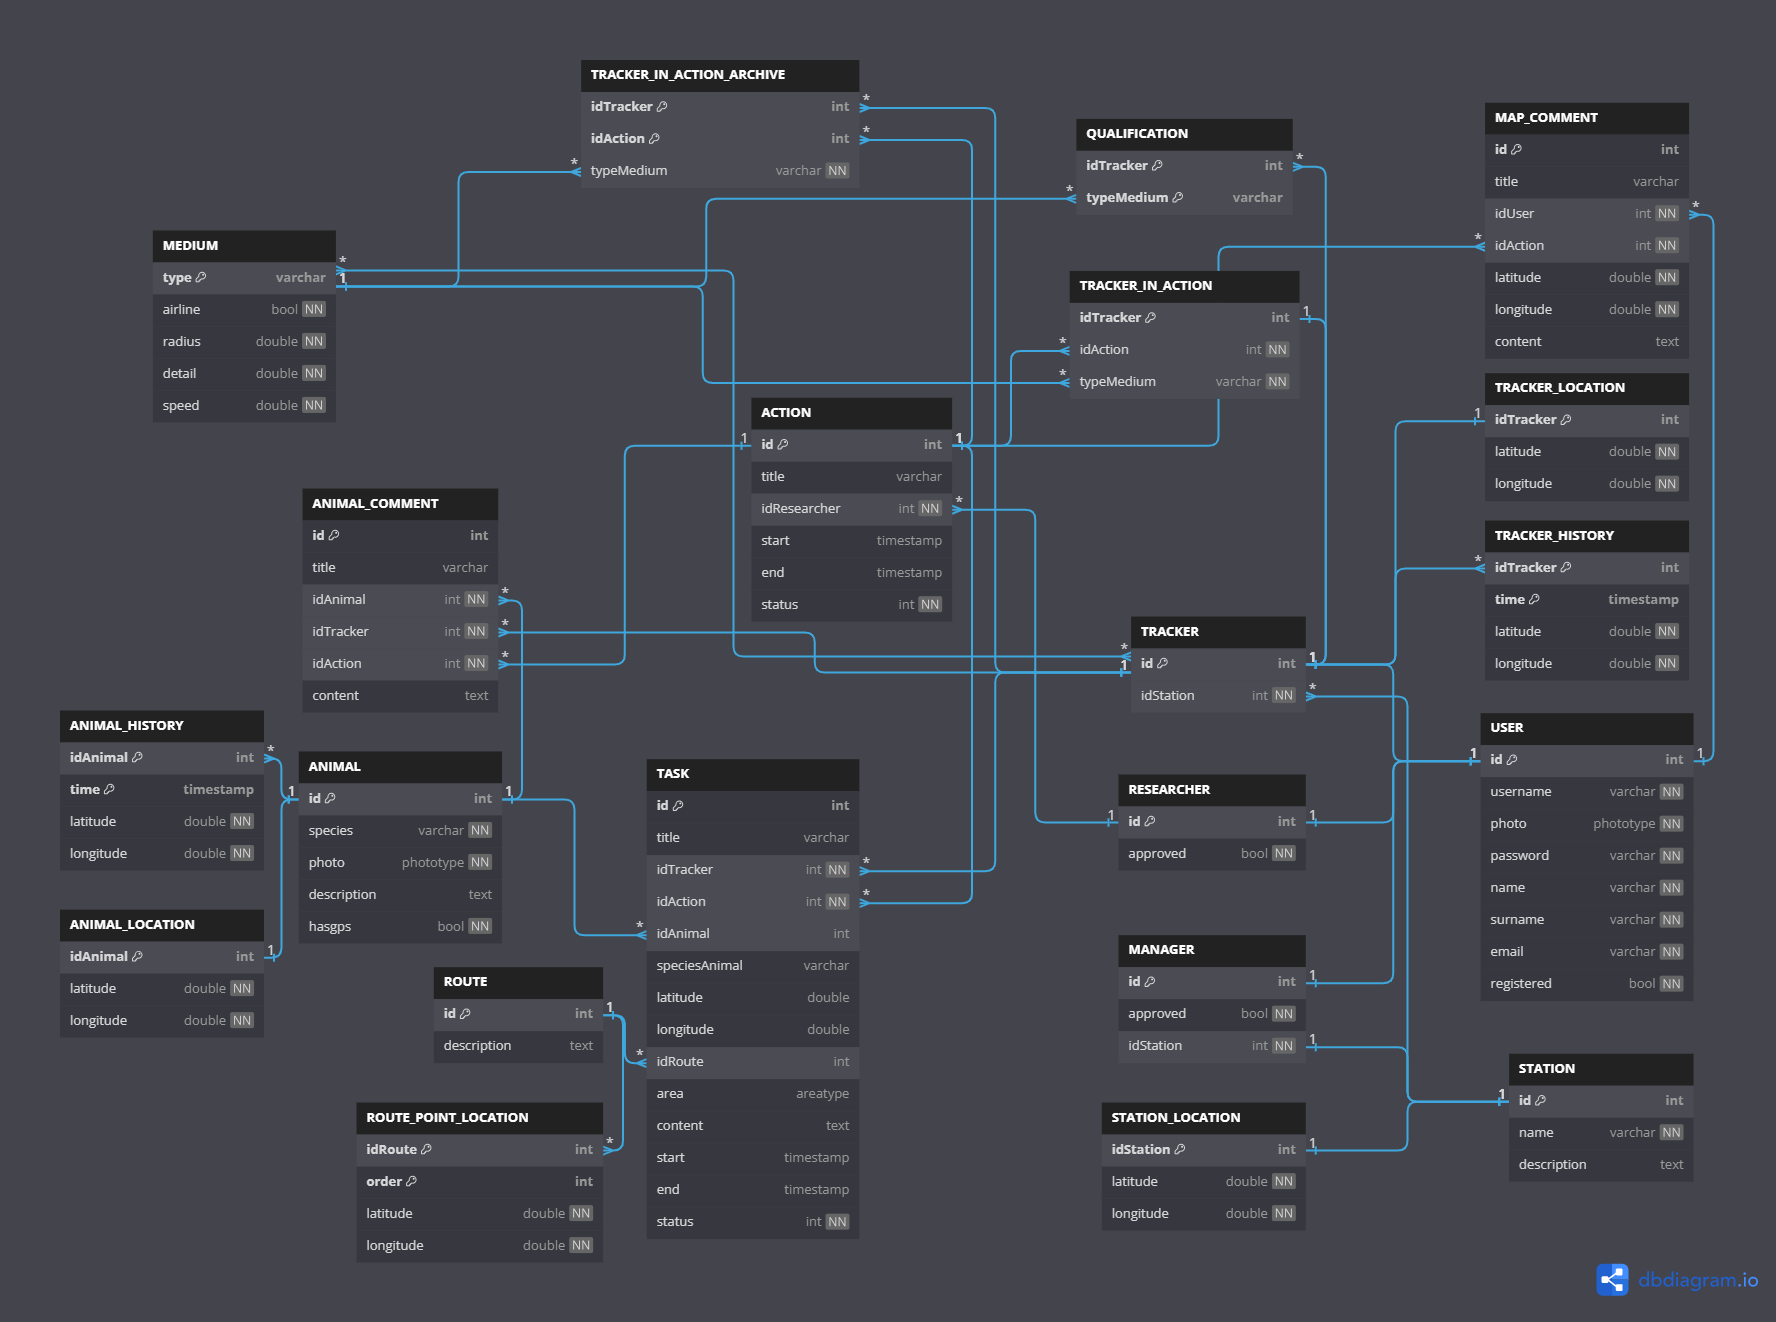
\includegraphics[scale=0.3]{slike/grafBaza.PNG} 
					% width=\textwidth,height=\textheight,keepaspectratio
					\centering
					\caption{E-R dijagram baze podataka}
					\label{fig:ERdiagram}
				\end{figure}				
				\restoregeometry
				
			\fi			
										
			
			\subsection{Dijagram baze podataka}			
			
				\vspace{12pt}						
				
				\begin{figure}[H] %ht
					\centering
					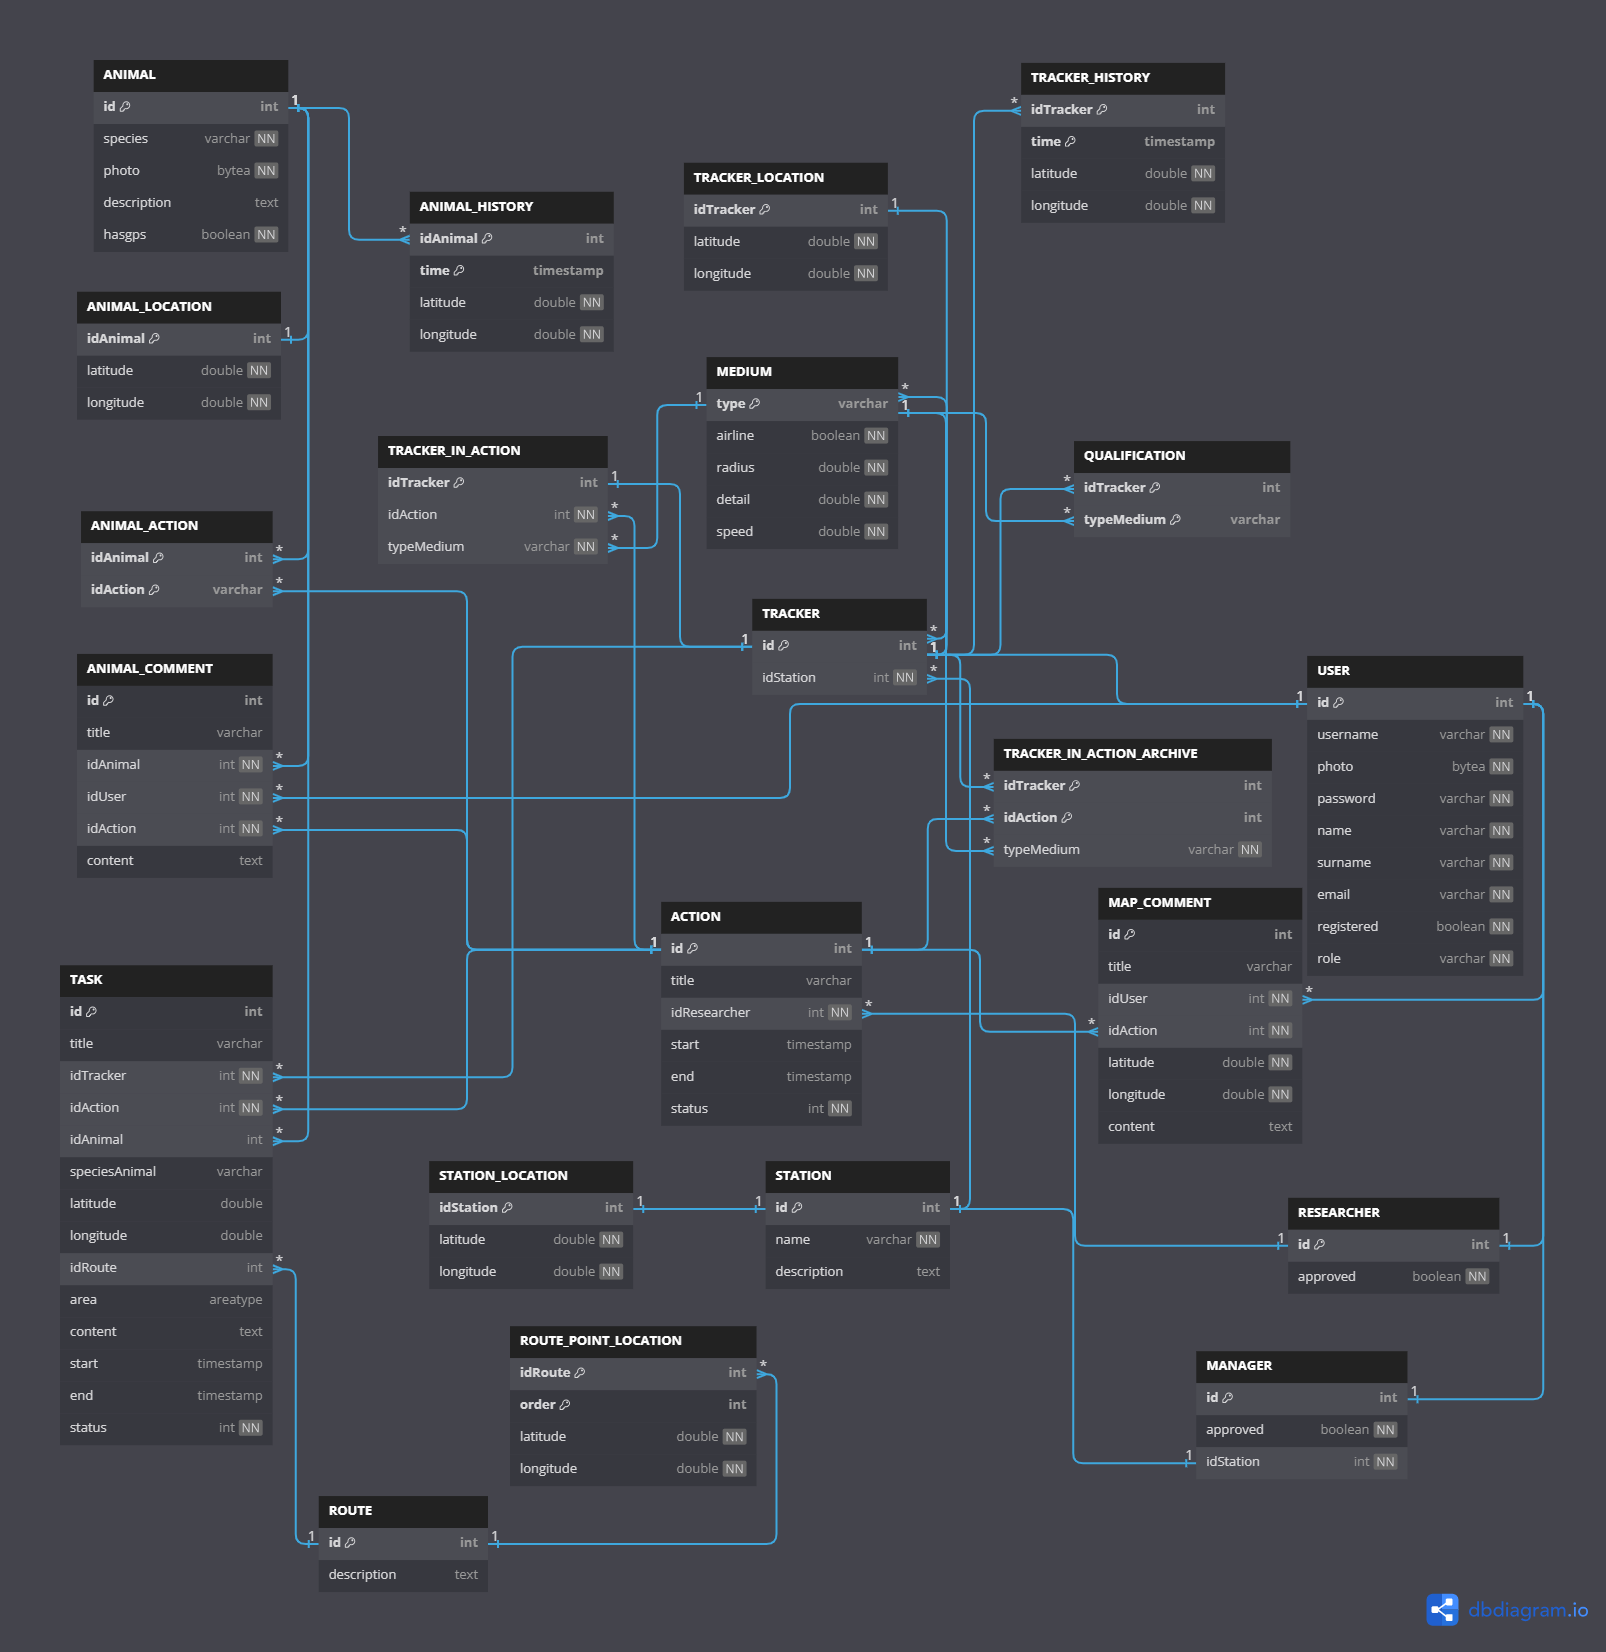
\includegraphics[width=\textwidth]{slike/baza.PNG}
					\caption{E-R dijagram baze podataka}
					\label{fig:ERdiagram}
				\end{figure}																												
																																	
			\eject
						
			
			
		\section{Dijagram razreda}
		
		\iffalse	\textit{Potrebno je priložiti dijagram razreda s pripadajućim opisom. Zbog preglednosti je moguće dijagram razlomiti na više njih, ali moraju biti grupirani prema sličnim razinama apstrakcije i srodnim funkcionalnostima.}\\
			
			\textbf{\textit{dio 1. revizije}}\\
			
			\textit{Prilikom prve predaje projekta, potrebno je priložiti potpuno razrađen dijagram razreda vezan uz \textbf{generičku funkcionalnost} sustava. Ostale funkcionalnosti trebaju biti idejno razrađene u dijagramu sa sljedećim komponentama: nazivi razreda, nazivi metoda i vrste pristupa metodama (npr. javni, zaštićeni), nazivi atributa razreda, veze i odnosi između razreda.}\\
			
			\textbf{\textit{dio 2. revizije}}\\			
			
			\textit{Prilikom druge predaje projekta dijagram razreda i opisi moraju odgovarati stvarnom stanju implementacije}
		\fi
			Na slikama 4.4, 4.5 i 4.6 prikazani su razredi koji pripadaju backend dijelu MVC arhitekture. Razredi prikazani na slici 4.3 nasljeđuju Controller razred. Metode implementirane u tim razredima obrađuju zahtjeve aktora koji dolaze s frontend servera obavljajući potrebne manipulacije podacima i šaljući odgovarajuće odgovore. Metode u Controller razredima obično vraćaju podatke u JSON formatu, a HTTP status kodovi koriste se za signalizaciju statusa zahtjeva (npr., uspješan odgovor, greška, itd.). Radi lakše organizacije, razredi su logički podijeljeni prema pravu pristupa metodama određenih aktera kako bi se smanjila prenapučenost unutar dijagrama. Prikazane su samo ovisnosti između razreda koji pripadaju istom dijelu dijagrama. Iz naziva i tipova atributa u razredima može se zaključiti vrsta ovisnosti među različitim razredima.Također se ponekad koriste dodatne DTO (Data transfer object) klase za specifične potrebe prijenosa podataka. Kod korištenja objekata koji predstavljaju modele ili DTO objekata u implementaciji selektivno se postavljaju atributi koji su potrebni za određene operacije, a ostali atributi su automatski postavljeni na null. To omogućuje modularno korištenje funkcija i zbog toga modeli i DTO objekti mogu imati reference na druge modele.
			
			\eject
		
			\vspace{12pt}						
			
			\begin{figure}[H] %ht
				\centering
				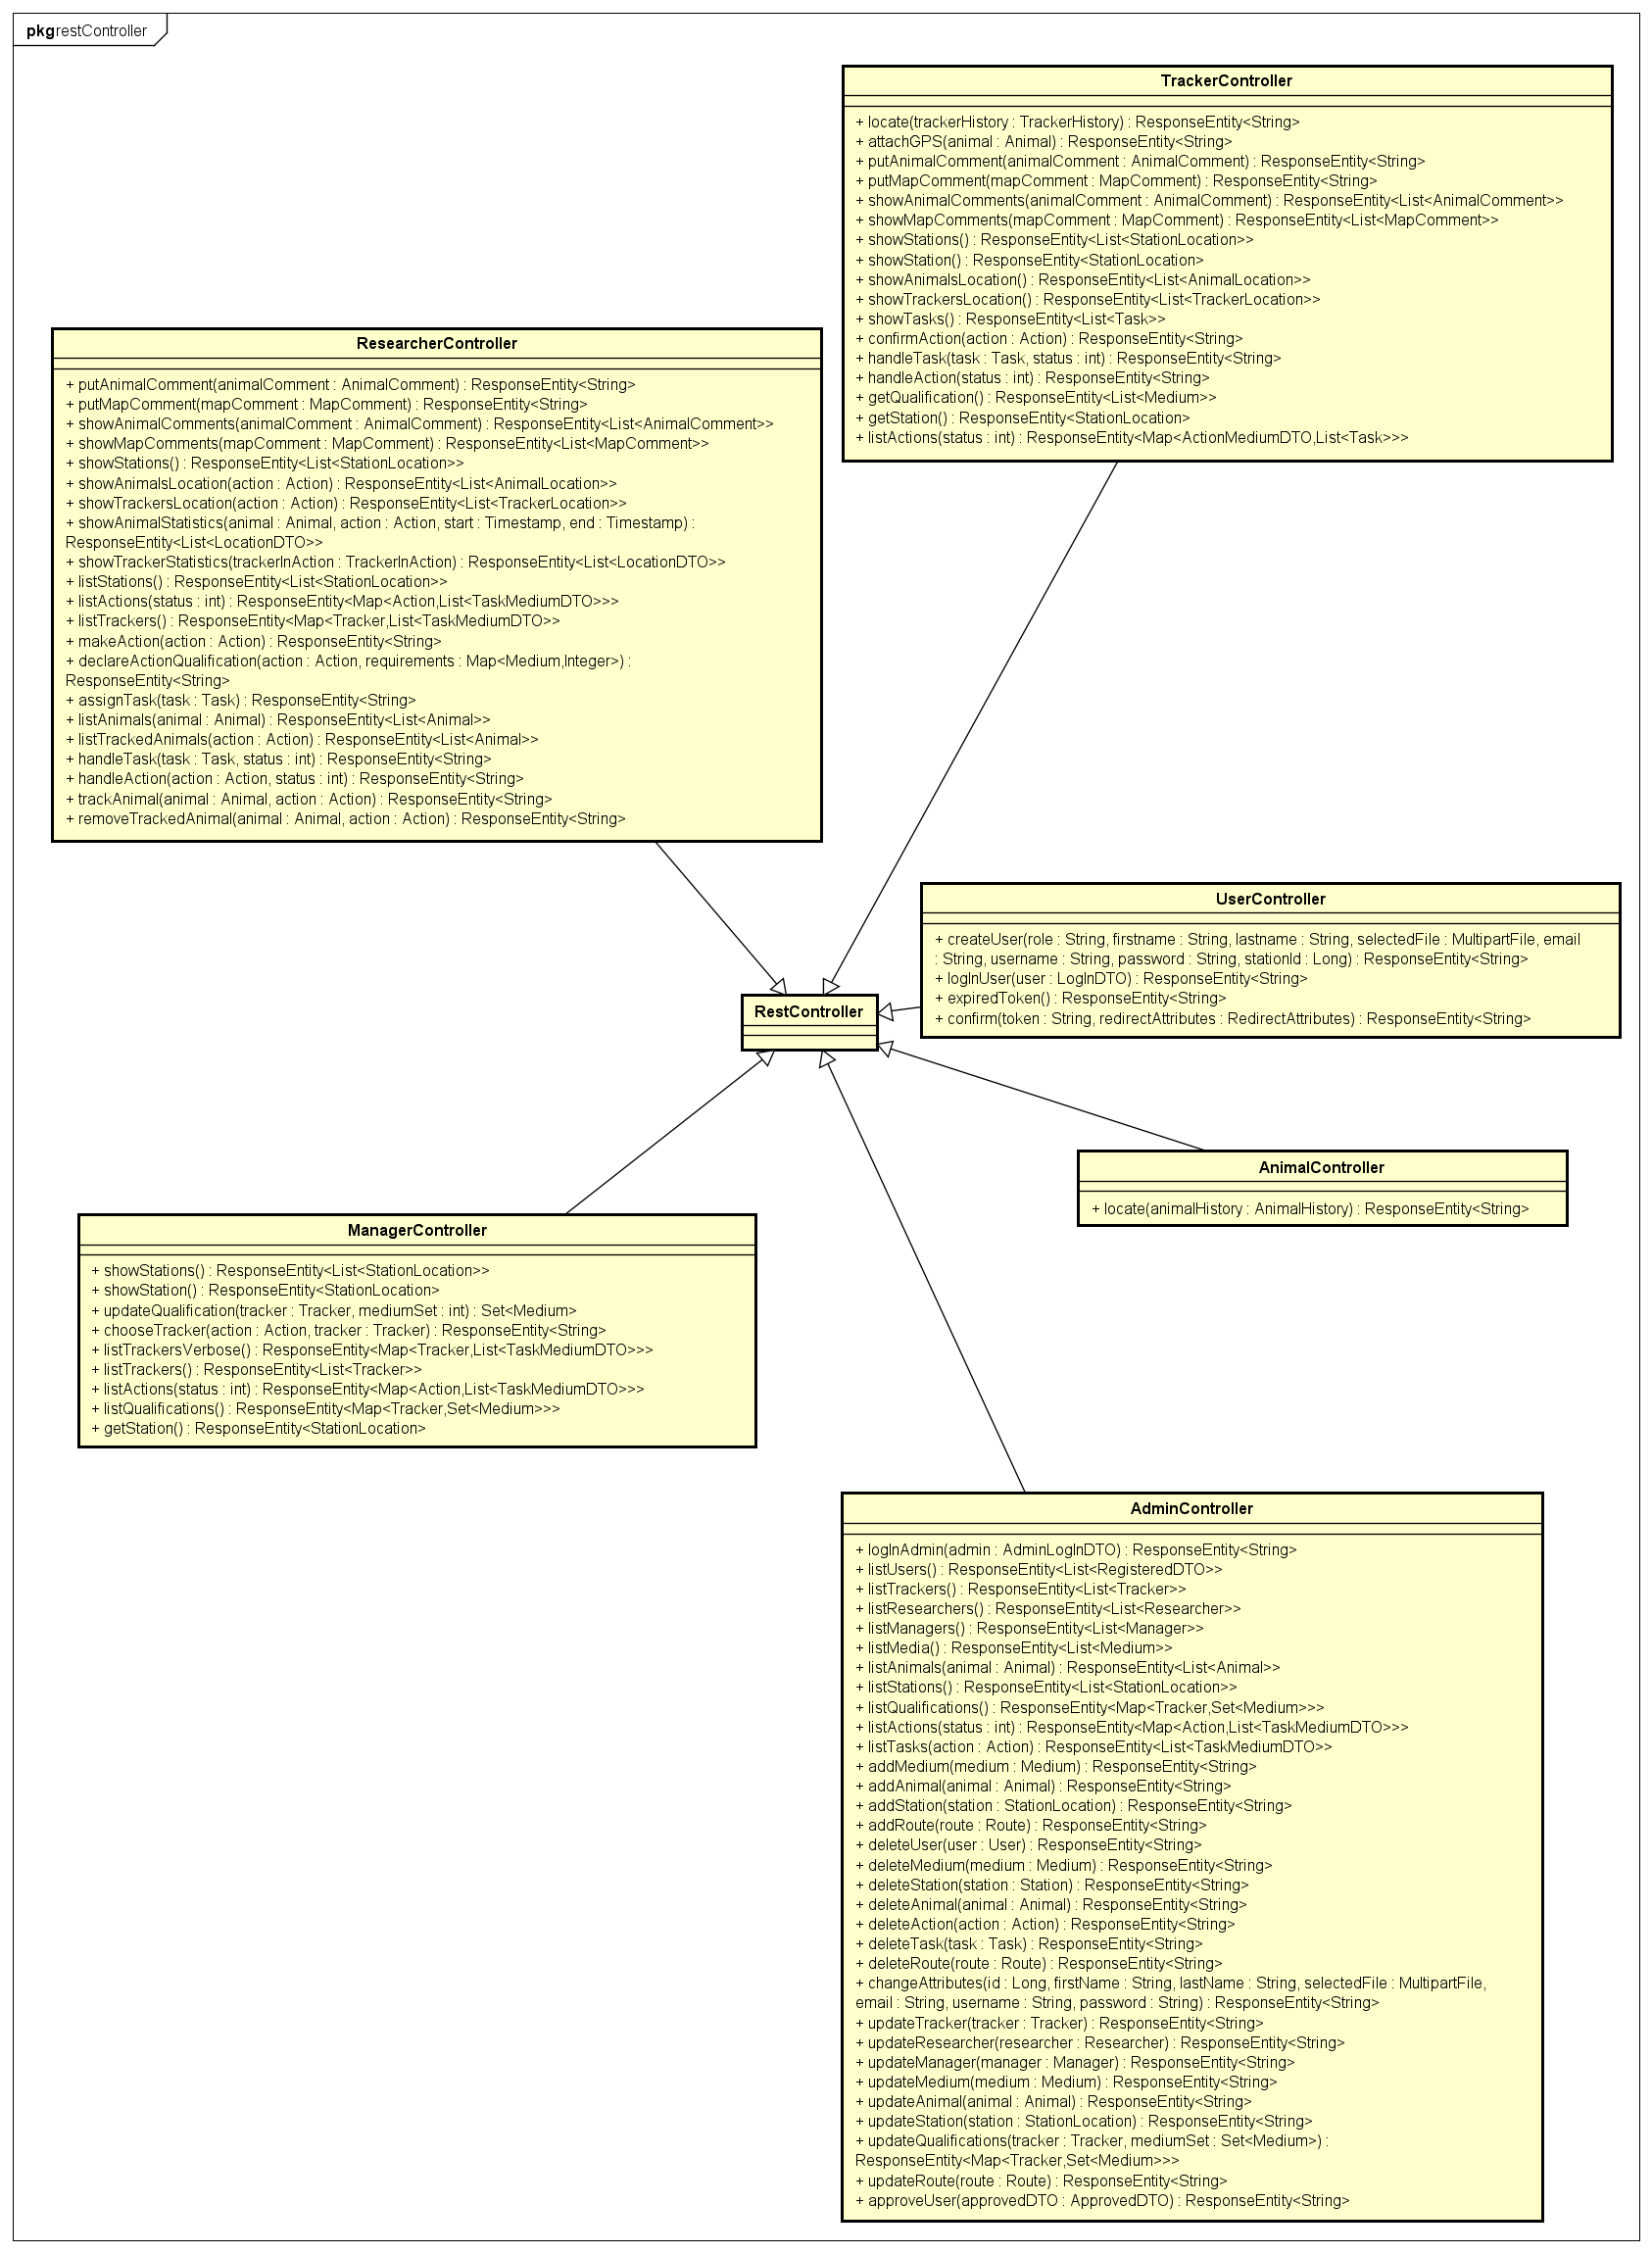
\includegraphics[width=\textwidth]{slike/controllerdiagram.png}
				\caption{Dijagram razreda - dio Controllers}
				\label{fig:Controllerdiagram}
			\end{figure}	
		
		\eject
		
		\begin{figure}[H] %ht
			\centering
			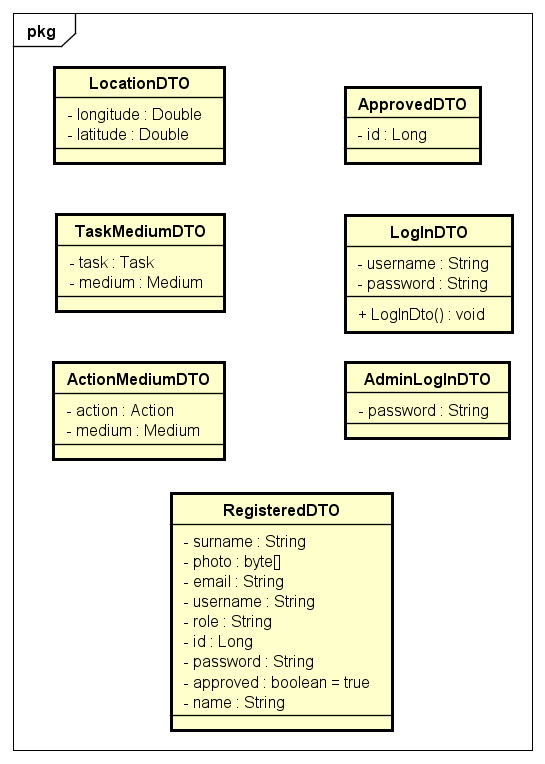
\includegraphics[width=\textwidth]{slike/dtodiagram.png}
			\caption{Dijagram razreda - dio Data transfer objects}
			\label{fig:DTOdiagram}
		\end{figure}
		
		\eject
		
		
		Model razredi preslikavaju strukturu baze podataka u aplikaciji. Svi entiteti realiziraju javne get i set metode za svoje privatne atribute. Modeli Researcher (istraživač), Tracker (tragač) i Manager (voditelj stanice) nasljeđuju model User (korisnik) te imaju svoje specifične atribute. Oni predstavljaju tri glavna tipa korisnika aplikacije od kojih svaki može upućivati specifične zahtjeve koji odražavaju mogućnosti tog tipa korisnika. Svaki korisnk se mora registrirati da bi koristio aplikaciju te korisnike tipa Researcher i Manager  administrator mora dodatno potvrditi. Istraživači organiziraju akcije s ciljem praćenja i prikupljanja podataka o životinjama, a na tim akcijama zadatke koje zadaje istraživač odrađuju tragači koji rade na toj akciji i pripadaju određenoj stanici koja ima svog voditelja koji odabire koji će tragači sudjelovati u nekoj akciji na temelju zahtjeva istraživača i kvalifikacija tragača. 
		
		\eject
		
		\begin{figure}[H] %ht
			\centering
			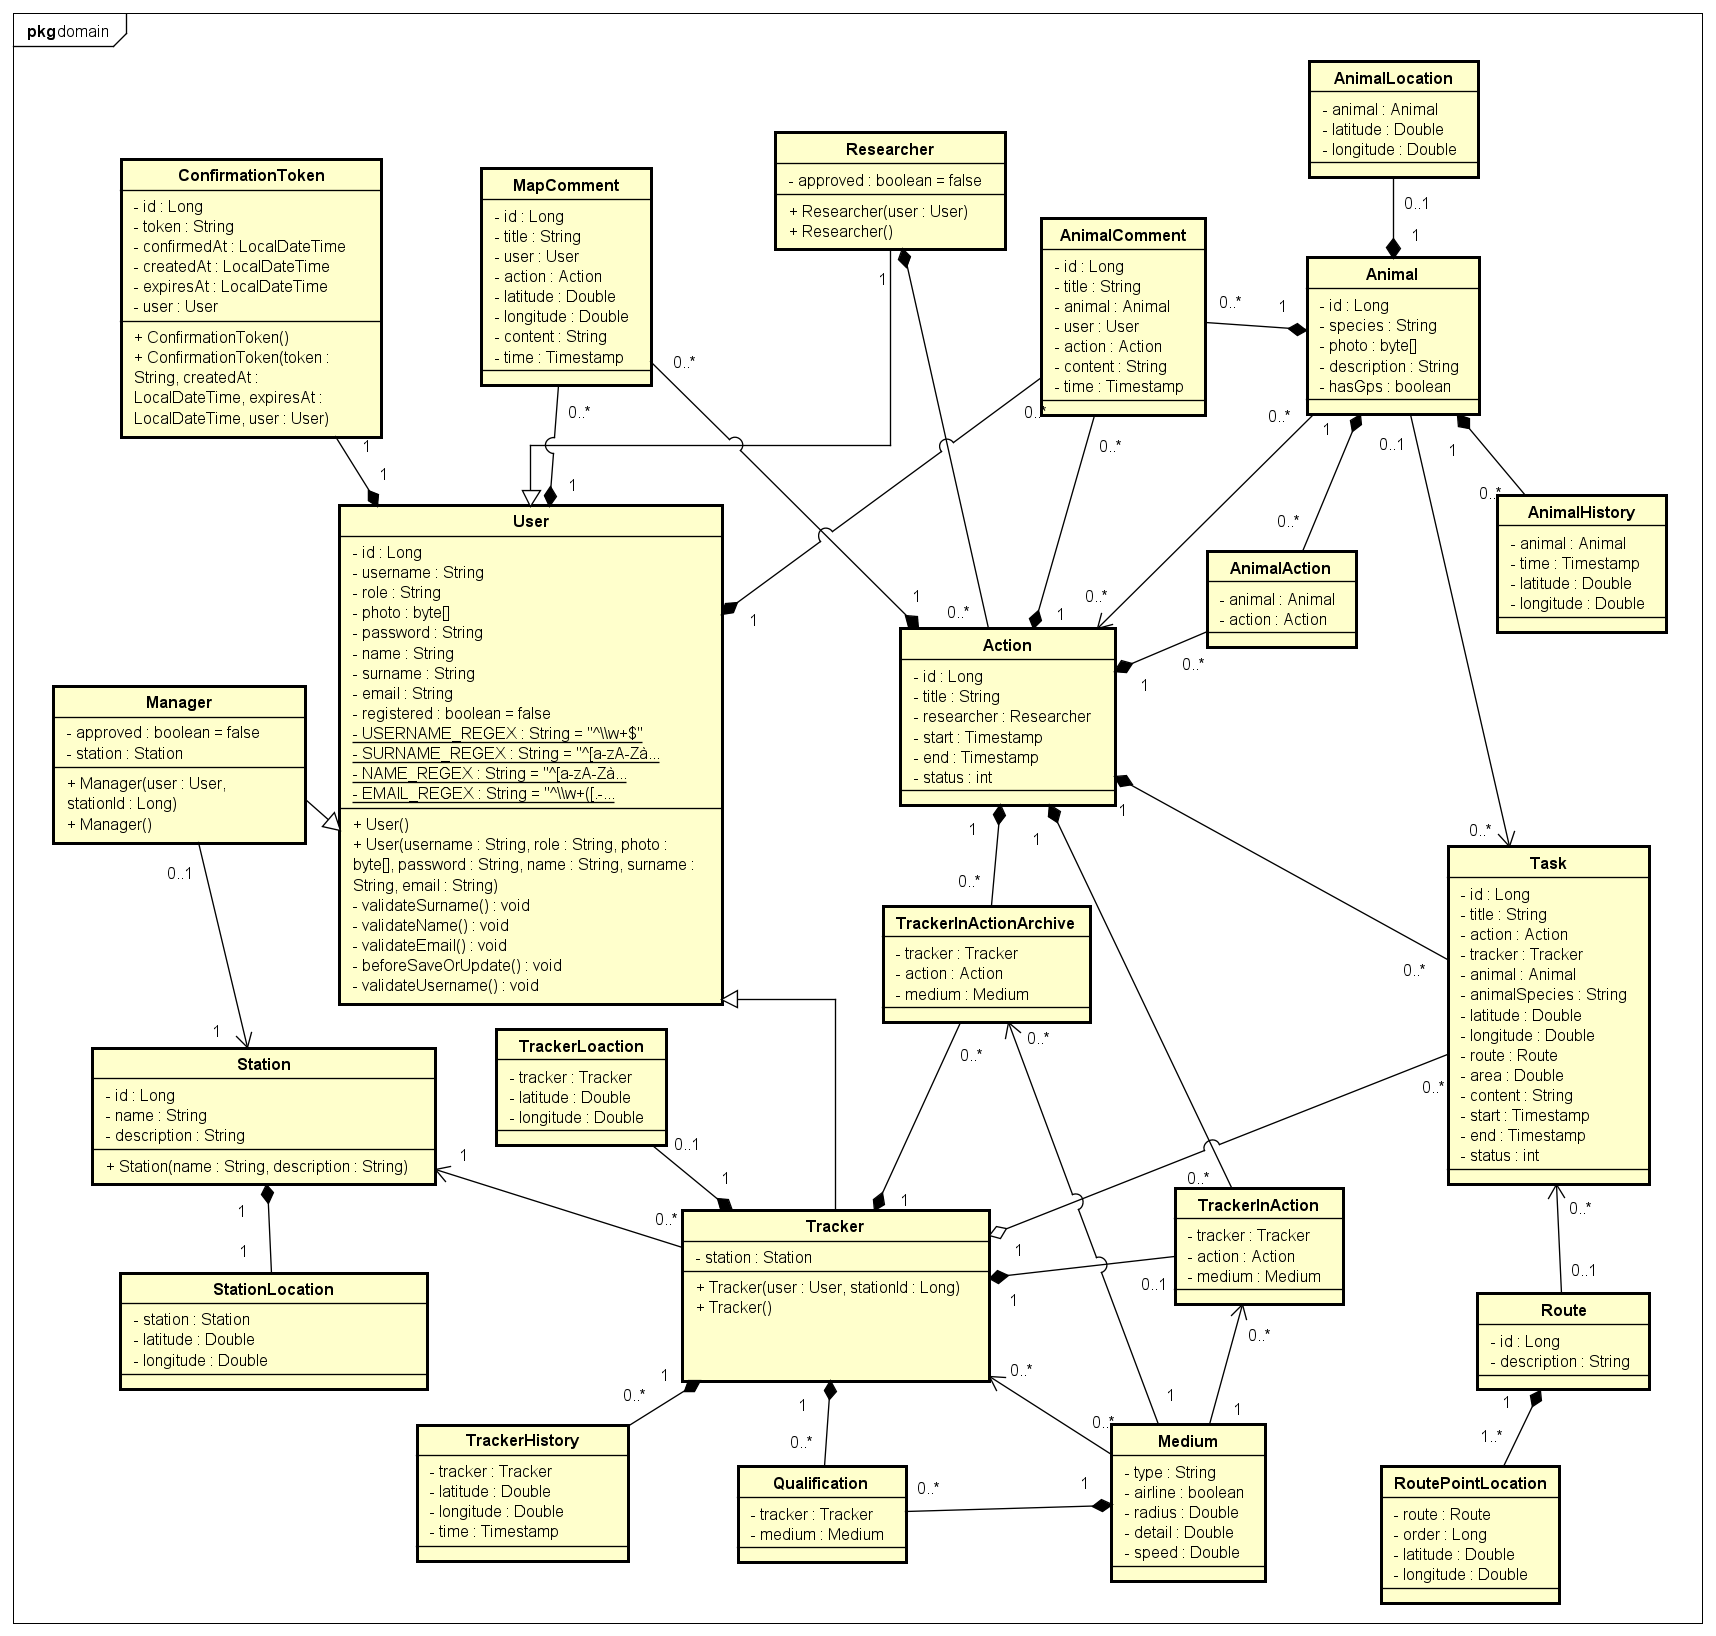
\includegraphics[width=\textwidth]{slike/modeldiagram.png}
			\caption{Dijagram razreda - dio Models}
			\label{fig:Modelrdiagram}
		\end{figure}
		
		\eject
		
		\section{Dijagram stanja}
			
			
			\noindent Dijagram stanja opisuje dinamičko ponašanje dijela sustava i prikazuje stanja objekata. Na slici ispod(slika 4.7) prikazuje se dijagram stanja za korisnika registriranog i ulogiranog kao Istraživač(Researcher).  Istraživaču se pokazuje početna stranica gdje ima mogućnost odabira 3 opcije: prikaza akcije, slanja zahtjeva za tragača i kreiranja nove akcije. Pri prikazu akcije istraživač može pogledati životinje koje se traže u akciji i može pogledati koji tragači su aktivni u akciji. Istraživač može popuniti zahtjev za tragača koji mu je potreban u akcijama i poslati ga na uvid voditelju. Novu akciju istraživač dodaje tako da klikne na dugme „create actions“, odabere tip akcije, odabere zadatke za svakog tragača i na kraju kreira akciju. Istraživač se može odjaviti u svakom trenutku.
			
			\begin{figure}[H]
				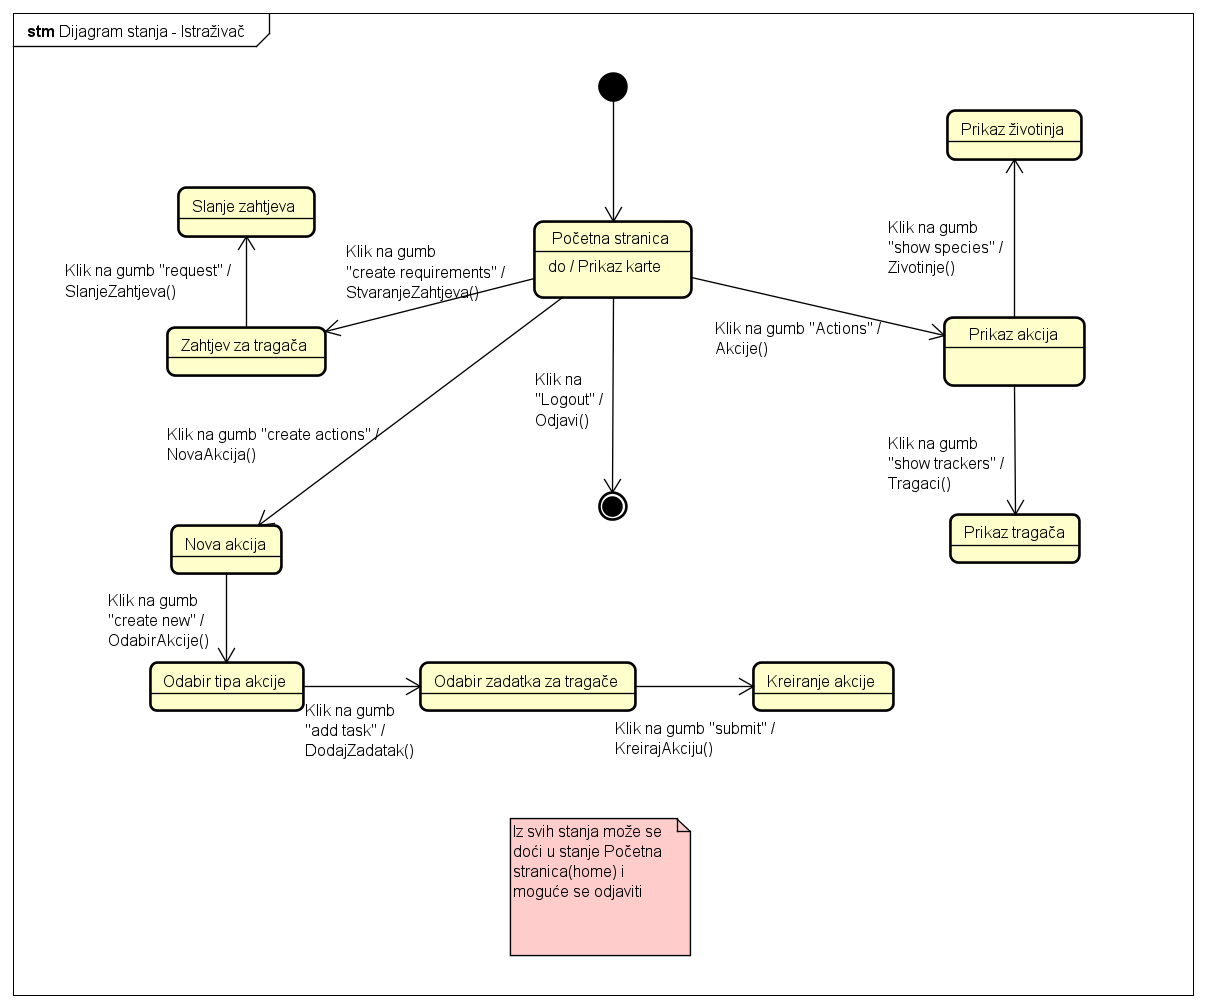
\includegraphics[scale=0.5]{slike/dijagram_stanja.PNG} %veličina slike u odnosu na originalnu datoteku i pozicija slike
				\centering
				\caption{Dijagram stanja}
				\label{fig:promjene}
			\end{figure}
			
			\eject 
		
		\section{Dijagram aktivnosti}
			
			\noindent Dijagram aktivnosti koristi se za opis modela toka upravljanja. Svaki korak u dijagramu odvija se nakon prethodno završenog te je dijagram vrlo čitljiv i lako razumljiv. Na slici ispod(slika 4.8) prikazan je dijagram aktivnosti za proces odabira podataka za prikazivanje na karti. Nakon što se korisnik prijavi u sustav, prikazuje mu se karta. Na njoj može odabrati opciju prikaza tragača ili opciju prikaza životinja. Aplikacija prikazuje željene podatke te korisnik nakon toga može odabrati prikaz toplinske karte i aplikacija mu to prikazuje.
			
			\begin{figure}[H]
				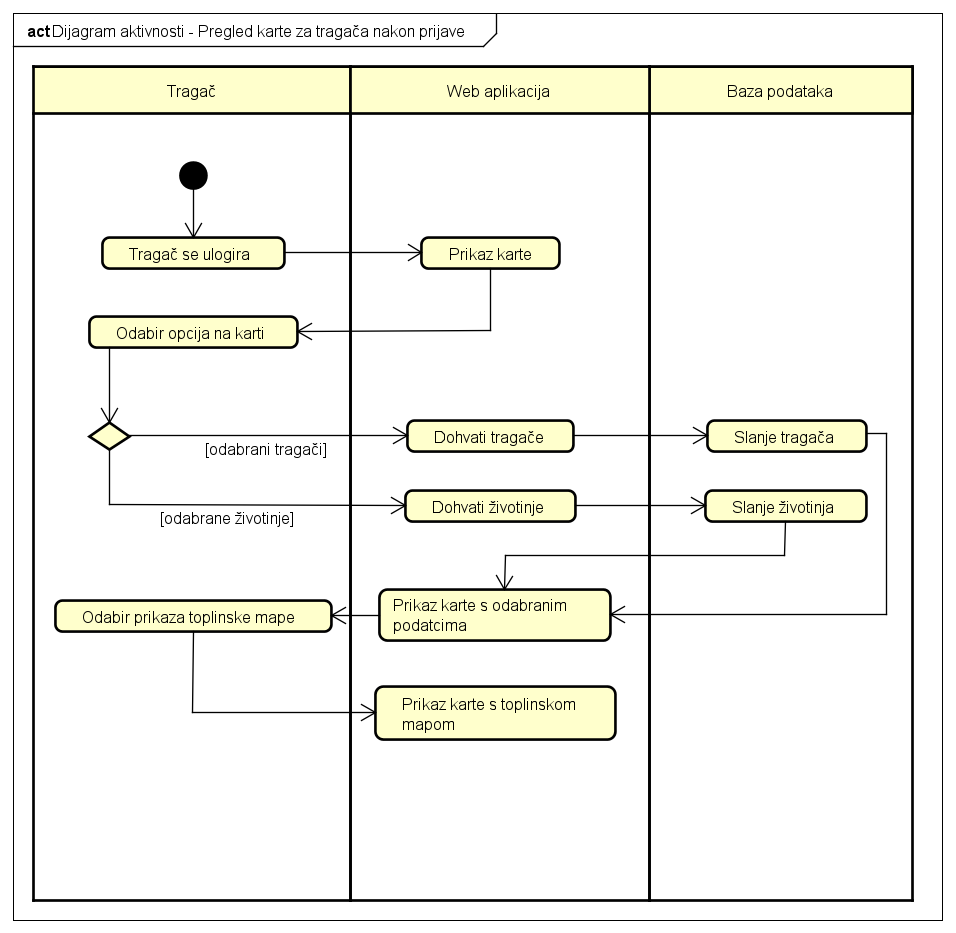
\includegraphics[scale=0.6]{slike/dijagram_aktivnosti.PNG} %veličina slike u odnosu na originalnu datoteku i pozicija slike
				\centering
				\caption{Dijagram aktivnosti}
				\label{fig:promjene}
			\end{figure}
			
			\eject
		\section{Dijagram komponenti}
		
			\noindent Dijagram komponenti opisuje organizaciju i međuovisnost komponenti, interne strukture i odnose prema okolini. Na slici ispod prikazan je dijagram sustava aplikacije WildTrack. Sustavu se pristupa preko dva sučelja. Pomoću sučelja za dohvat HTML, CSS i JS datoteka poslužuju se datoteke potrebne za frontend dio aplikacije. Pomoću router komponente, koja je dio Reacta, određuje se koje će se datoteke poslati na sučelje aplikacije.  Na frontendu se nalaze JavaScript datoteke koje zajedno čine razne komponente nazvane po aktorima kojima se pristupa. Preko sučelja za dohvat podataka u JSON obliku pristupa se REST API komponenti koja poslužuje podatke s backend dijela aplikacije. Hibernate komponenta dohvaća podatke iz SQL baze podataka te ih prosljeđuje DTO-u. Controller komponenta zadužena je primanje upita i odlučuje što se uzima od DTO komponente. React-view komponenta komunicira s aplikacijom i prikazuje potrebne podatke ovisno o zahtjevima.
			
			\begin{figure}[H]
				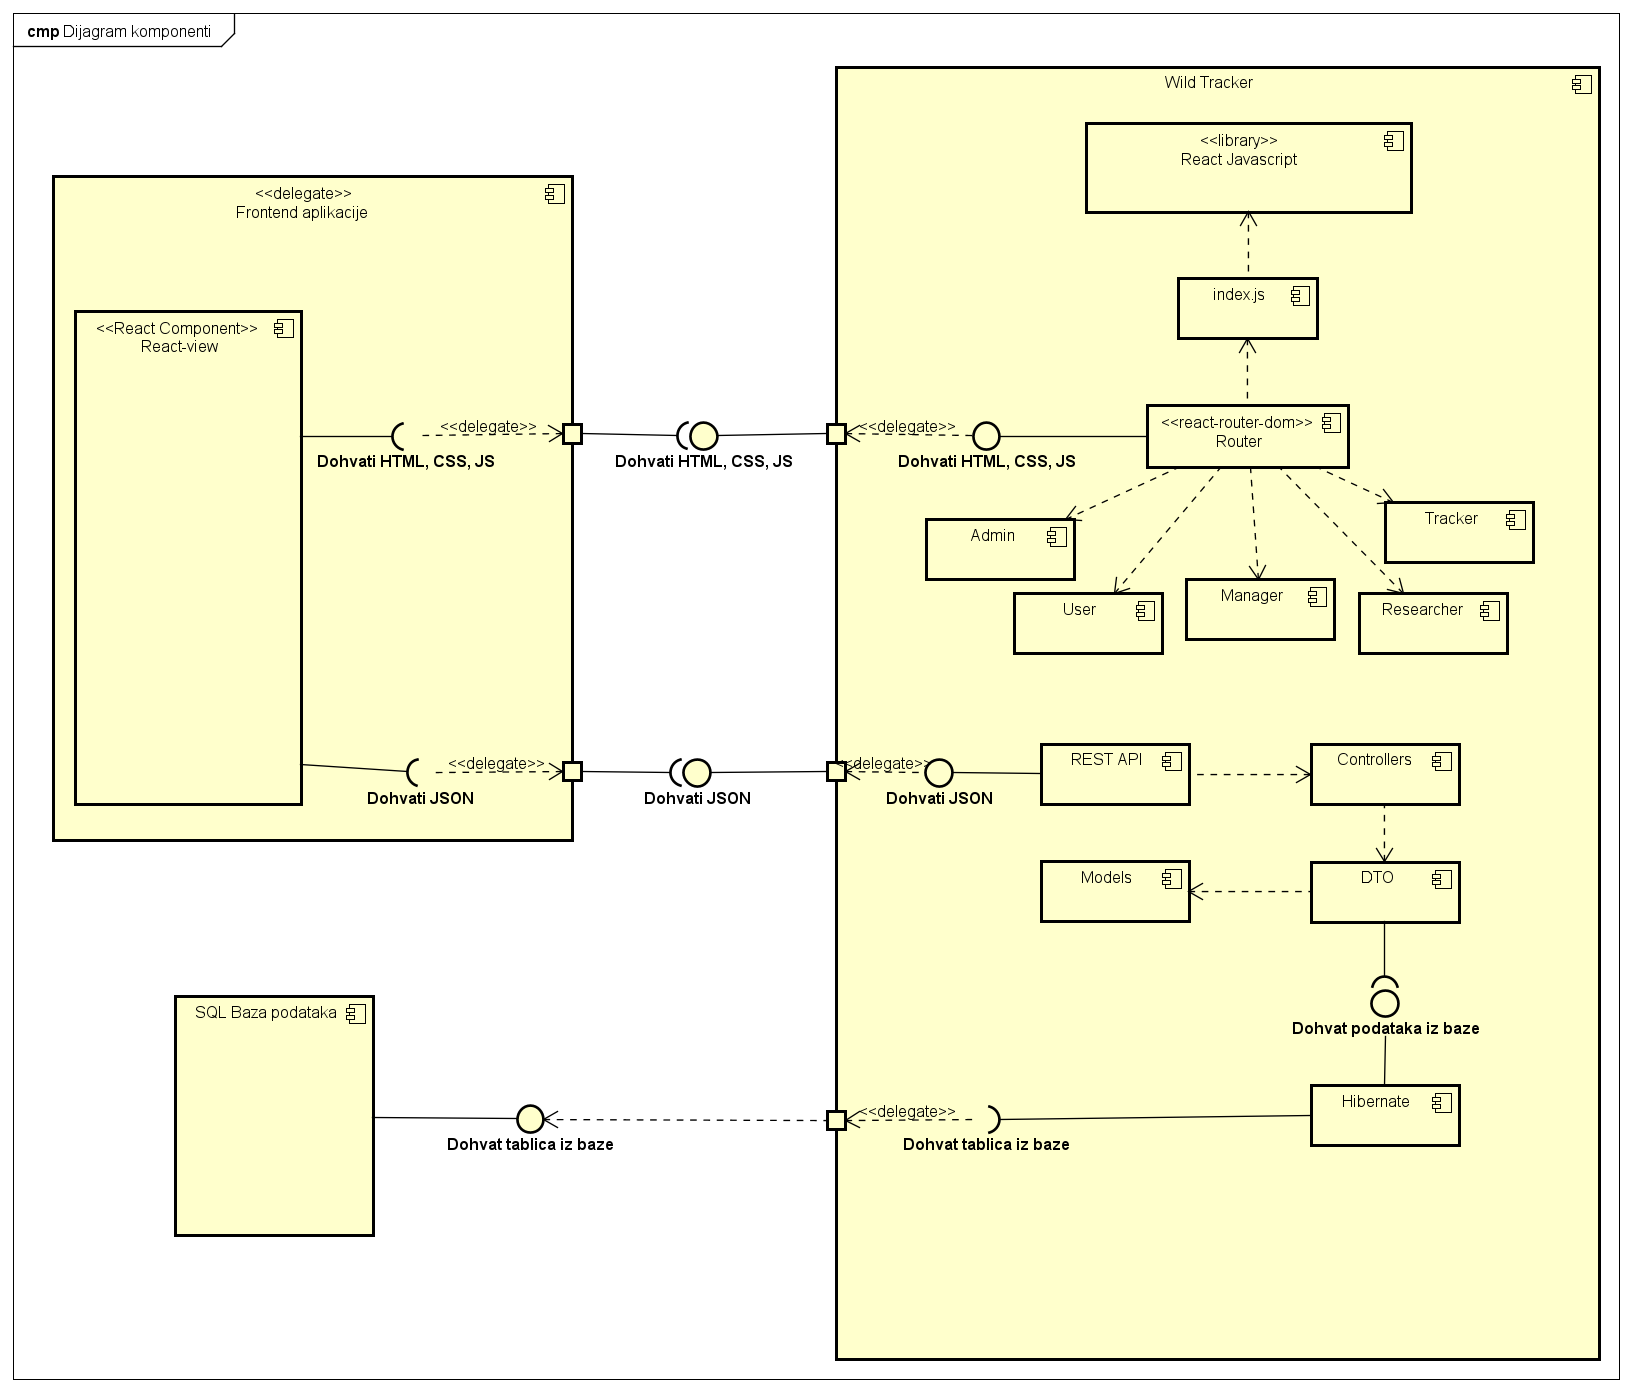
\includegraphics[scale=0.4]{slike/dijagram_komponenti.PNG} %veličina slike u odnosu na originalnu datoteku i pozicija slike
				\centering
				\caption{Dijagram komponenti}
				\label{fig:promjene}
			\end{figure}